\documentclass [aspectratio=169]{beamer}
\usetheme{Boadilla}
\usepackage{textpos} % package for the positioning
\usepackage[]{graphicx}
\usepackage{graphicx}
\usepackage{float}
\usepackage{hyperref}
\usepackage{caption}
\usepackage{subcaption}
\usepackage{algorithm,algpseudocode}
\usepackage[export]{adjustbox}
\usepackage{tikz}
\usetikzlibrary{positioning}
\usetikzlibrary{arrows, shapes, decorations, automata, backgrounds, fit, petri, calc}
\setbeamertemplate{itemize items}[circle]
\setbeamertemplate{enumerate items}[circle]
\setbeamertemplate{itemize subitem}{$\triangleright$}


\newcommand*{\logofont}{\fontfamily{phv}\selectfont}
\definecolor{uoftblue}{RGB}{6,41,88} % official blue color for uoft

\vspace{1in}
\title[]{DoSS Summer Bootcamp Probability \\ Module 1}
\author[]{Ichiro Hashimoto}
\institute[]{University of Toronto}
\date{July 8, 2024}

% set color
\setbeamercolor{title in head/foot}{bg=white}
\setbeamercolor{author in head/foot}{bg=white}
\setbeamercolor{date in head/foot}{fg=uoftblue}
\setbeamercolor{date in head/foot}{bg=white}
\setbeamercolor{title}{fg=uoftblue}
\setbeamerfont{title}{series=\bfseries}
\setbeamercolor{frametitle}{fg=uoftblue}
\setbeamerfont{frametitle}{series=\bfseries}
\setbeamercolor*{item}{fg=uoftblue}
\setbeamercolor{block title}{bg=uoftblue}
\setbeamercolor{block title}{fg=white}
\setbeamercolor{block body}{bg=uoftblue!5!white}

% set logo at non-title pages
\logo{
\includegraphics[height=0.8cm]{logo_uoft.png}\vspace*{-.055\paperheight}\hspace*{.85\paperwidth}}

% set margin
\setbeamersize{text margin left=10mm,text margin right=10mm}

\newcommand{\mc}{\mathcal}

\begin{document}
{
\setbeamertemplate{logo}{}
\begin{frame}
    \vspace{0.5in}
    \titlepage
    \begin{textblock*}{4cm}(0.5cm,-7.5cm)
        
\includegraphics[width=4cm]{logo_uoft.png}
    \end{textblock*}
    \begin{textblock*}{8cm}(5.0cm,-7cm)
        \huge \color{uoftblue}{$\Bigr\rvert$ \hspace{0.15cm} \textbf{\logofont Statistical Sciences}}
    \end{textblock*}
\end{frame}
}

\begin{frame}{Roadmap}
\textbf{A bridge connecting undergraduate probability and graduate probability}\\
\vspace{0.2in}
\uncover<1->{
\textbf{Undergraduate-level probability}
\begin{itemize}
    \item Concrete; 
    \item Examples and scenarios;
    \item Rely on computation...
\end{itemize}}
\vspace{0.1in}
\uncover<2->{
\textbf{Graduate-level probability}
\begin{itemize}
    \item Abstract (measure theory); 
    \item Laws and properties;
    \item Rely on construction and inference... 
\end{itemize}}
\end{frame}

\begin{frame}{Roadmap}
\begin{figure}
    \centering
    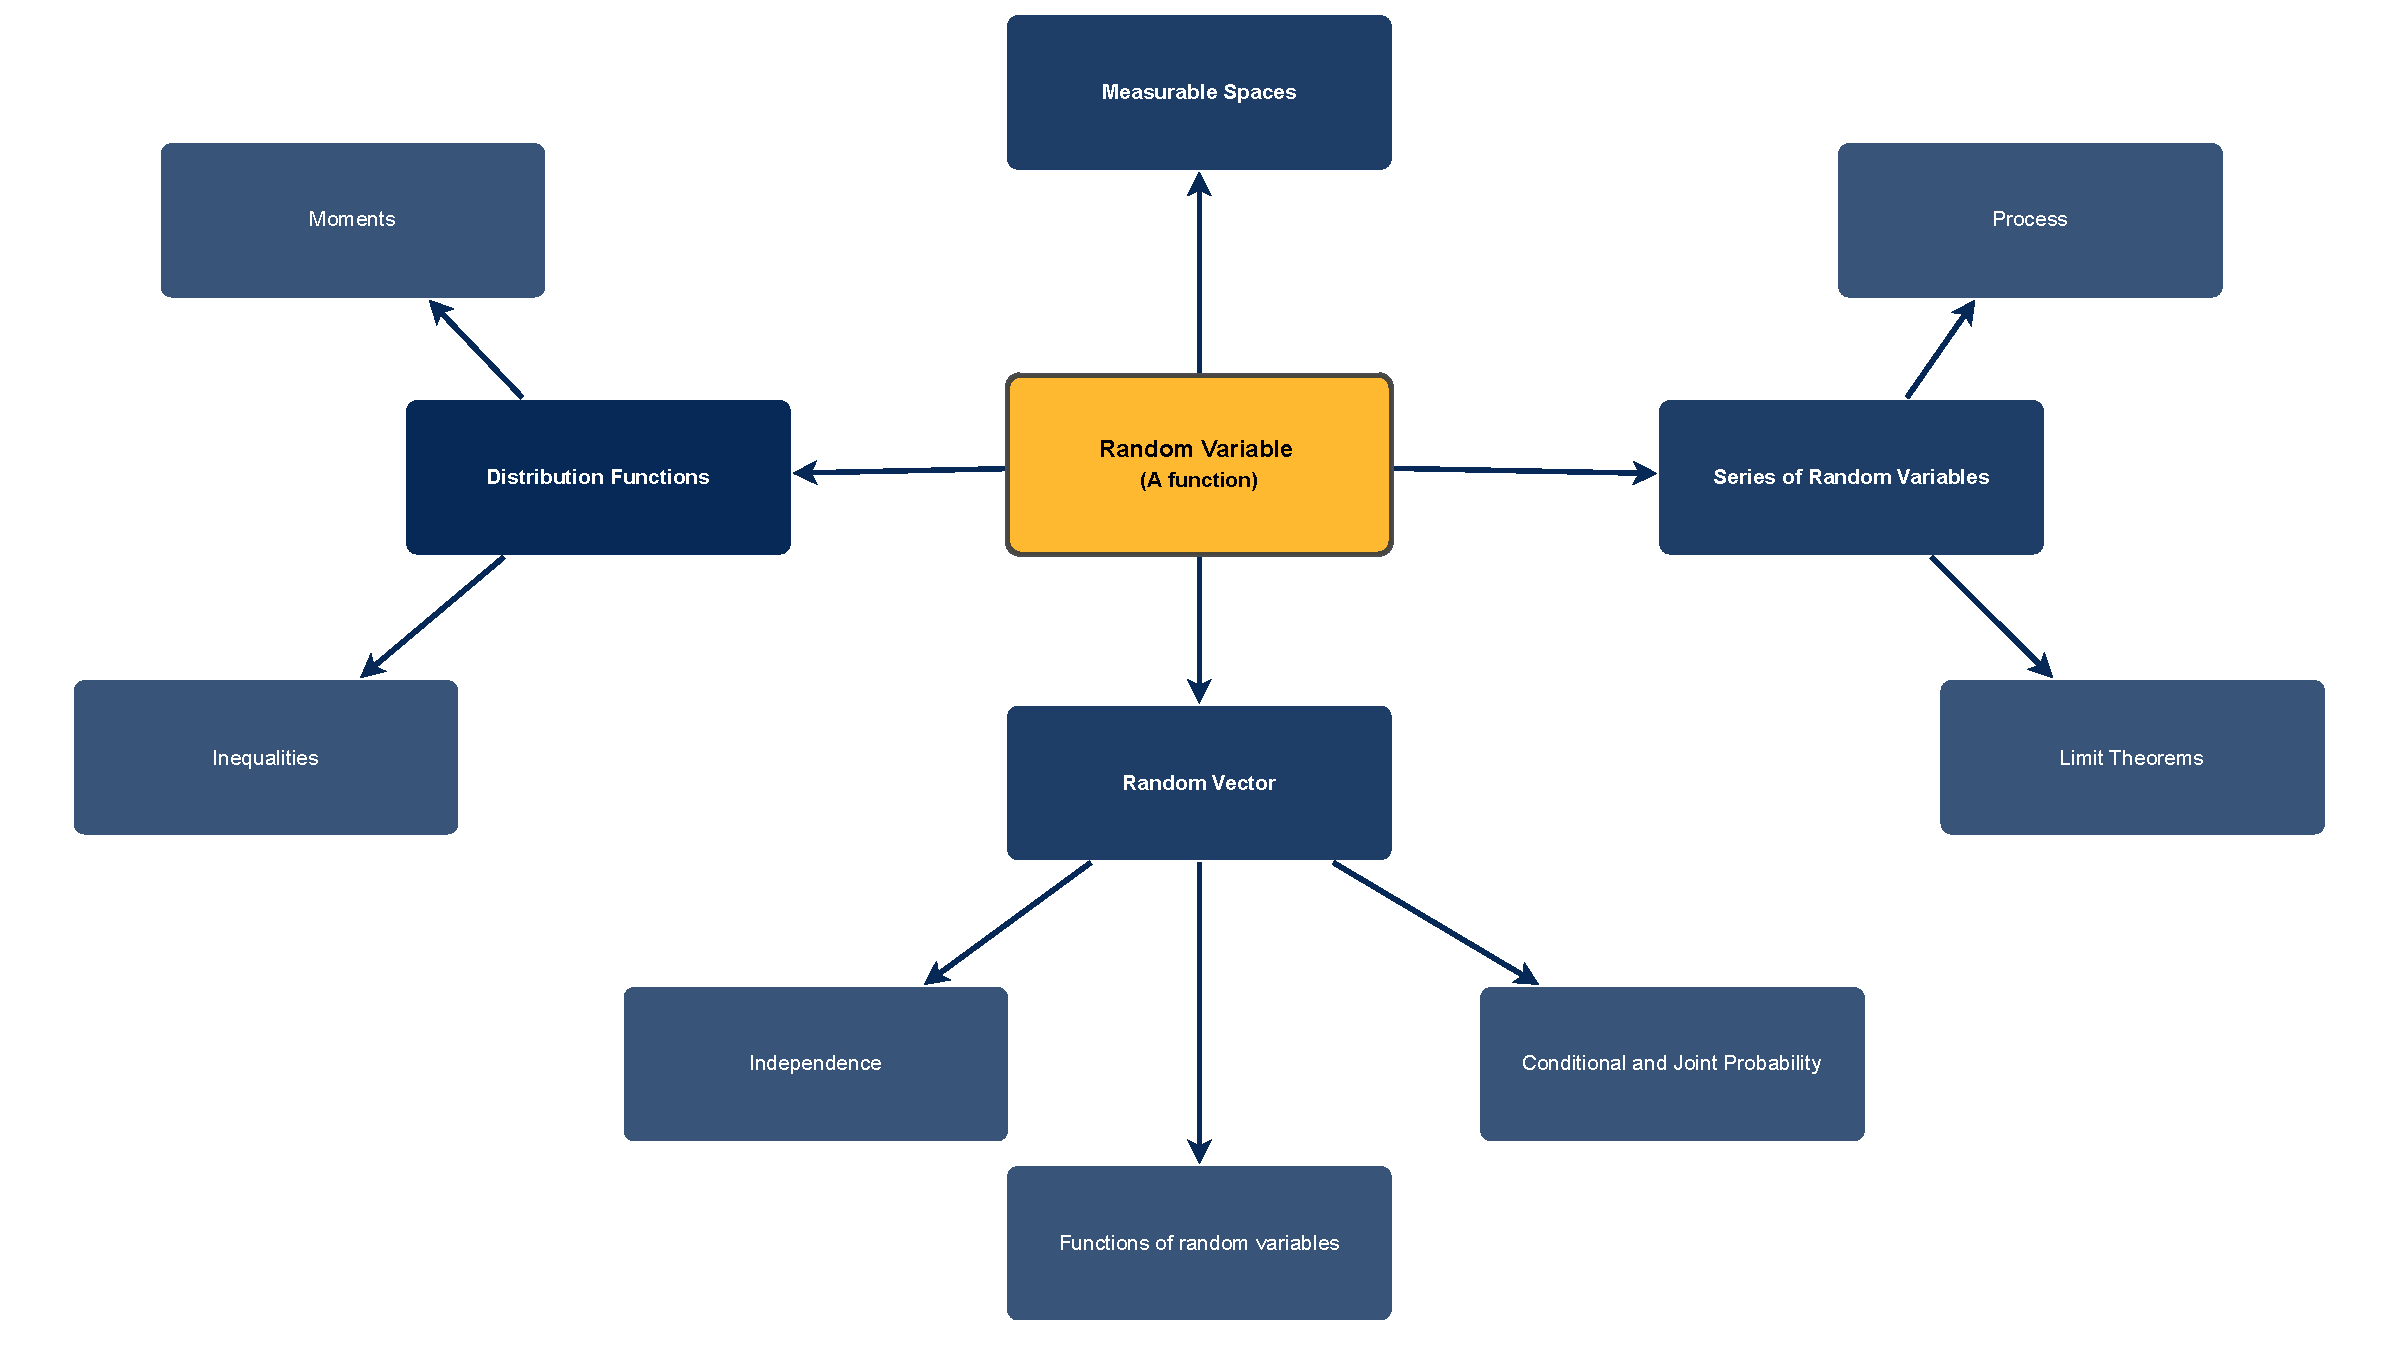
\includegraphics[width = 0.85\textwidth]{Roadmap.pdf}
    \caption{Roadmap}
    \label{fig:my_label}
\end{figure}
\end{frame}

\begin{frame}{Outline}
    \begin{itemize}
        \item Measurable spaces
        \begin{itemize}
            \item Sample Space
            \item $\sigma$-algebra
        \end{itemize}
        \item Probability measures
              \begin{itemize}
            \item Measures on $\sigma$-field
            \item Basic results
        \end{itemize}
        \item Conditional probability
        \begin{itemize}
            \item Bayes’ rule
            \item Law of total probability

        \end{itemize}
    \end{itemize}
\end{frame}

% Think about the very simple scenario of tossing a coin. If we toss the coin again and again, a very intuitive action is to count how many heads we have and how many tails we have. And soon you would be thinking, is the number of heads significantly larger? And this tells us something about the physical property of the coin: does it tend to land on heads or tails? And we describe the tendency by defining the probability 



\begin{frame}{Measurable spaces}
    \begin{block}{Sample Space}
    The sample space $\Omega$ is the set of all possible outcomes of an experiment.
    \end{block}
    \textbf{Examples:}
    \begin{itemize}
        \item Toss a coin: $\{H, T\}$
        \item Roll a die: $\{1, 2, 3, 4, 5, 6\}$
    \end{itemize}
    \uncover<2->{
    \begin{block}{Event}
    An event is a collection of possible outcomes (subset of the sample space).
    \end{block}
    \textbf{Examples:}
    \begin{itemize}
        \item Get head when tossing a coin: $\{H\}$
        \item Get an even number when rolling a die: $\{2, 4, 6\}$
    \end{itemize}}
\end{frame}

\begin{frame}{Measurable spaces}
    \begin{block}{$\sigma$-algebra}
  A $\sigma$-algebra ($\sigma$-field) $\mc{F}$ on $\Omega$ is a non-empty collection of subsets of $\Omega$ such that
    \begin{itemize}
        \item If $A \in \mc{F}$, then $A^c \in \mc{F}$, %close on counter set
        \item If $A_1, A_2, \cdots \in \mc{F}$, then $\cup_{i = 1}^\infty A_i \in \mc{F}$. %close on countable union
    \end{itemize}
    \end{block}
    \textbf{Remark:} $\varnothing, \Omega \in \mc{F}$
    \vspace{1.5in}
\end{frame}

\begin{frame}{Probability measures}
    \begin{block}{Measures on $\sigma$-field}
    A function $\mu: \mc{F} \to R^{+}\cup \{+\infty\}$ is called a measure if
    \begin{itemize}
        \item $\mu(\varnothing) = 0$,
        \item If $A_1, A_2, \cdots \in \mc{F}$ and $A_i \cap A_j = \varnothing$, then $\mu(\cup_{i = 1}^\infty A_i) = \sum_{i = 1}^\infty \mu(A_i)$.
    \end{itemize}
    If $\mu(\Omega) = 1$, then $\mu$ is called a probability measure. 
    \end{block}
    \vspace{0.1in}
    \uncover<2->{
    \textbf{Properties:}\\
    \begin{itemize}
        \item Monotonicity: $A \subseteq B \quad \Rightarrow  \quad \mu(A) \le \mu(B)$
        \item Subadditivity: $A \subseteq  \cup_{i = 1}^\infty A_i \quad \Rightarrow  \quad \mu(A) \le \sum_{i = 1}^\infty \mu(A_i)$
        \item Continuity from below: $A_i \nearrow A \quad \Rightarrow  \quad \mu(A_i) \nearrow \mu(A)$
        \item Continuity from above: $A_i \searrow A$ and $\mu(A_i) < \infty \quad \Rightarrow  \quad \mu(A_i) \searrow \mu(A)$
    \end{itemize}}
\end{frame}

\begin{frame}{Probability measures}
    \textbf{Proof of continuity from below:}
\vspace{2.5in}
\end{frame}

\begin{frame}{Probability measures}
    \textbf{Proof of continuity from above:}
\vspace{1.5in}\\
\textbf{Remark:} $\mu(A_i) < \infty$ is vital. %provide a counterexample
\vspace{1in}
\end{frame}


\begin{frame}{Probability measures}
\textbf{Examples:}\\
\vspace{0.1in}
$\Omega = \{\omega_1, \omega_2, \cdots\}$, $A = \{\omega_{a_1}, \cdots, \omega_{a_i}, \cdots\}$ $\Rightarrow \mu(A) = \sum_{j = 1}^\infty \mu(\omega_{a_j})$.\\
Therefore, we only need to define $\mu(\omega_j) = p_j \ge 0$. \\
If further $\sum_{i = 1}^\infty p_j = 1$, then $\mu$ is a probability measure. 
\vspace{0.1in}
\begin{itemize}
    \item Toss a coin: \\
    \vspace{0.5in}
    \item Roll a die: 
    \vspace{0.5in}
\end{itemize}
\end{frame}

\begin{frame}{Conditional probability}
\vspace{0.1in}
\textbf{Original problem}:
\begin{itemize}
    \item What is the probability of some event $A$?
    \item $P(A)$ is determined by our probability measure.
\end{itemize}
\vspace{0.1in}
\textbf{New problem}:
\begin{itemize}
    \item Given that $B$ happens, what is the probability of some event $A$?
    \item $P(A \mid B)$ is the conditional probability of the event $A$ given $B$.
\end{itemize}
\vspace{0.1in}
\uncover<2->{
\textbf{Example:}
\begin{itemize}
    \item Roll a die: $P(\{2\} \mid {\text{even number}})$
    \vspace{1in}
\end{itemize}}
\end{frame}


\begin{frame}{Conditional probability}
    \begin{block}{Bayes' rule}
    $$P(A \mid B) = \dfrac{P(A\cap B)}{P(B)}, \quad P(B) > 0$$
    \end{block}
    \vspace{0.1in}
    \textbf{Remark:} Does conditional probability $P(\cdot \mid B)$ satisfy the axioms of a probability measure?
    \vspace{1.5in}
\end{frame}

\begin{frame}{Conditional probability}
\begin{block}{Multiplication rule}
$${P(A\cap B)} = P(A \mid B) P(B) = P(B \mid A) P(A)$$
\end{block}
\vspace{0.1in}
\textbf{Generalization}:
    \begin{block}{Law of total probability}
    Let $A_1, A_2, \cdots, A_n$ be a partition of $\omega$, such that $P(A_i) > 0$, then
    $$P(B) = \sum_{i = 1}^n P(A_i)P(B \mid A_i)$$
    \end{block}
    \vspace{1in}
\end{frame}

\begin{frame}{Problem Set}
    \textbf{Problem 1:} Prove that for a $\sigma$-field $\mc{F}$, if $A_1, A_2, \cdots \in \mc{F}$, then $\cap_{i = 1}^\infty A_i \in \mc{F}$.\\
    \vspace{0.1in}
    \textbf{Problem 2:} Prove monotonicity and subadditivity of measure $\mu$ on $\sigma$-field. \\
    \vspace{0.1in}
    \textbf{Problem 3:} (Monty Hall problem) Suppose you're on a game show, and you're given the choice of three doors: Behind one door is a car; behind the others, goats. You pick a door, say No. 1, and the host, who knows what's behind the doors, opens another door, say No. 3, which has a goat. He then says to you, "Do you want to pick door No. 2?" Is it to your advantage to switch your choice?\\
    (Assumptions: the host will not open the door we picked and the host will only open the door which has a goat.)
% Lecture 4 CMU

\end{frame}


\end{document}
